% !TEX root = BioInspired.tex

\chapter{Slides - Gray Scott}

\section{Problem}

	Generate the lambda, theta, alpha, and mu Gray-Scott patterns described in the slides.  These 

patterns are reminiscent of those found in nature, such as animal coat patterns as well as bacteria 

colonies.

	
\subsection{Solution}

Using the code provided by Dr. McGough, the Gray-Scott program was implemented in C due to 

performance issues with the python code.  The C code used to run this program is honestly confusing as 

hell to me... it just looks like a bunch of random calculations.  However, the data is then represented in a 

plot using Gnuplot.

\subsection{Issues}

Narrowing down the exact number for the F and K parameters was difficult.  This resulted in

some not exact matches to the slides in some cases, and in others it didn't resemble the slides at all.

\subsection{Analysis}

The patterns generated were not exact matches to the given templates.  It was hard to get the 

right values for F and K which is what caused the differences.  It was pretty amazing to see how little 

changes affected the final product in a huge way.

\begin{figure}[tbh]
\begin{center}
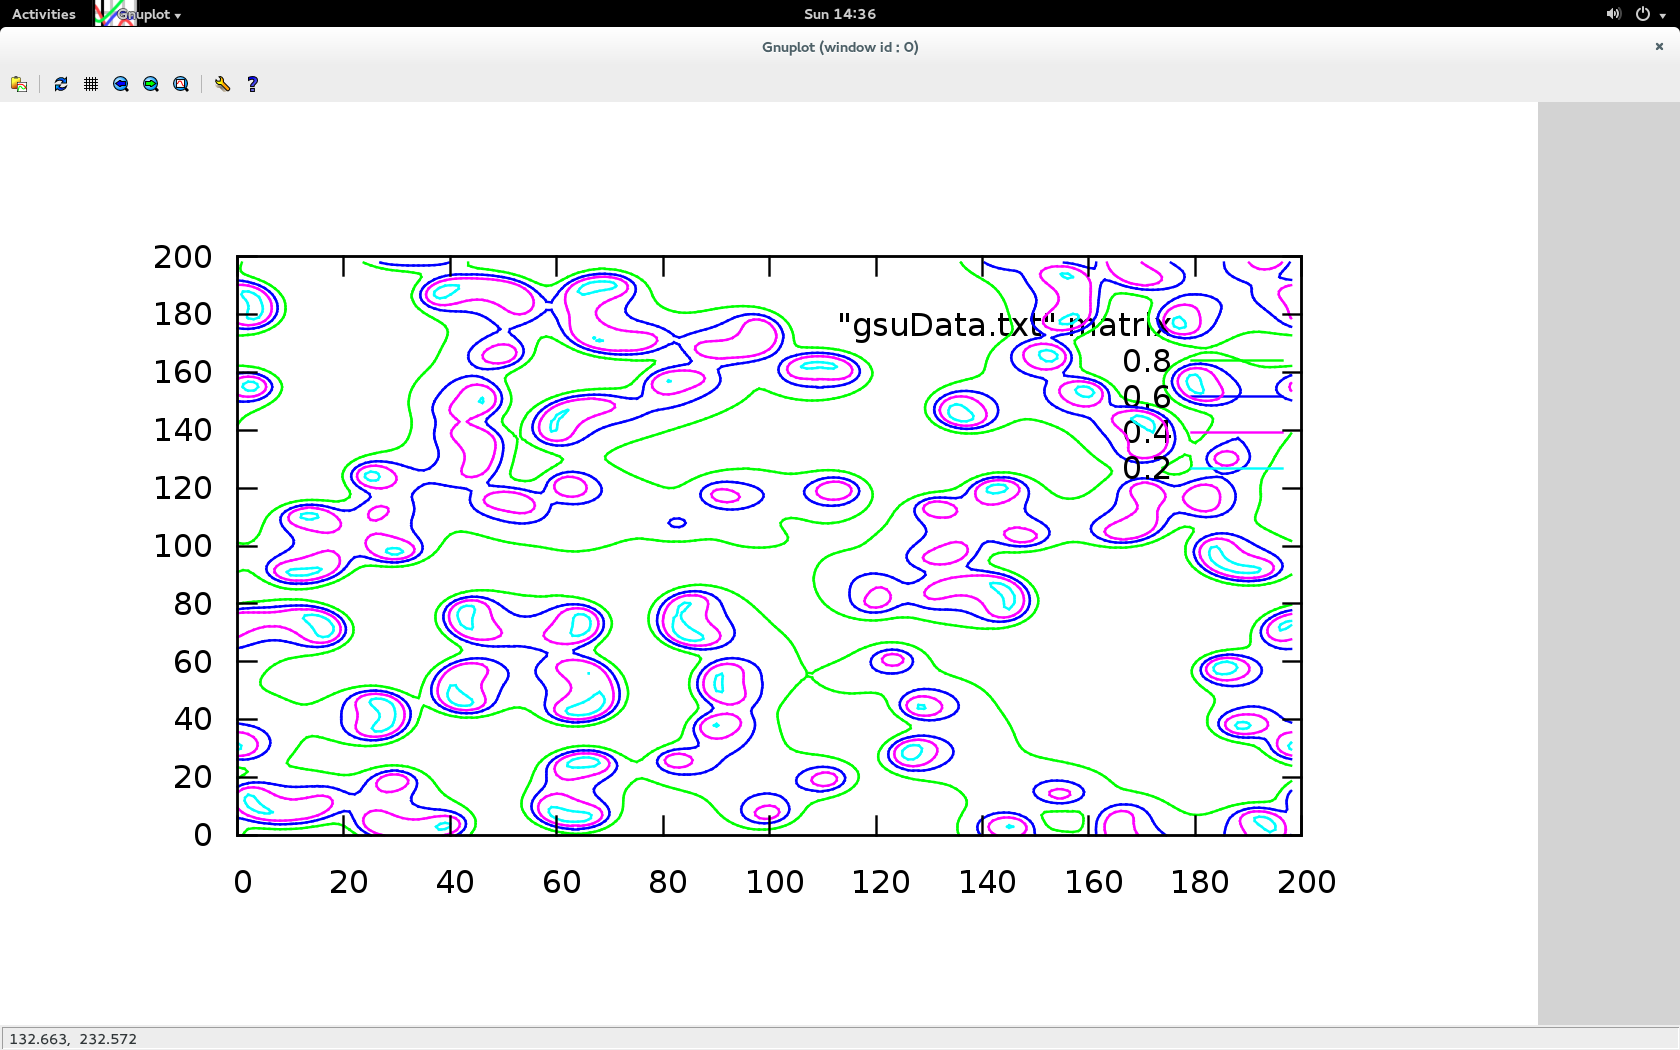
\includegraphics[width=0.75\textwidth]{alpha.png}
\end{center}
\caption{Alpha\label{fig:gprun}}
\end{figure}

\begin{figure}[tbh]
\begin{center}
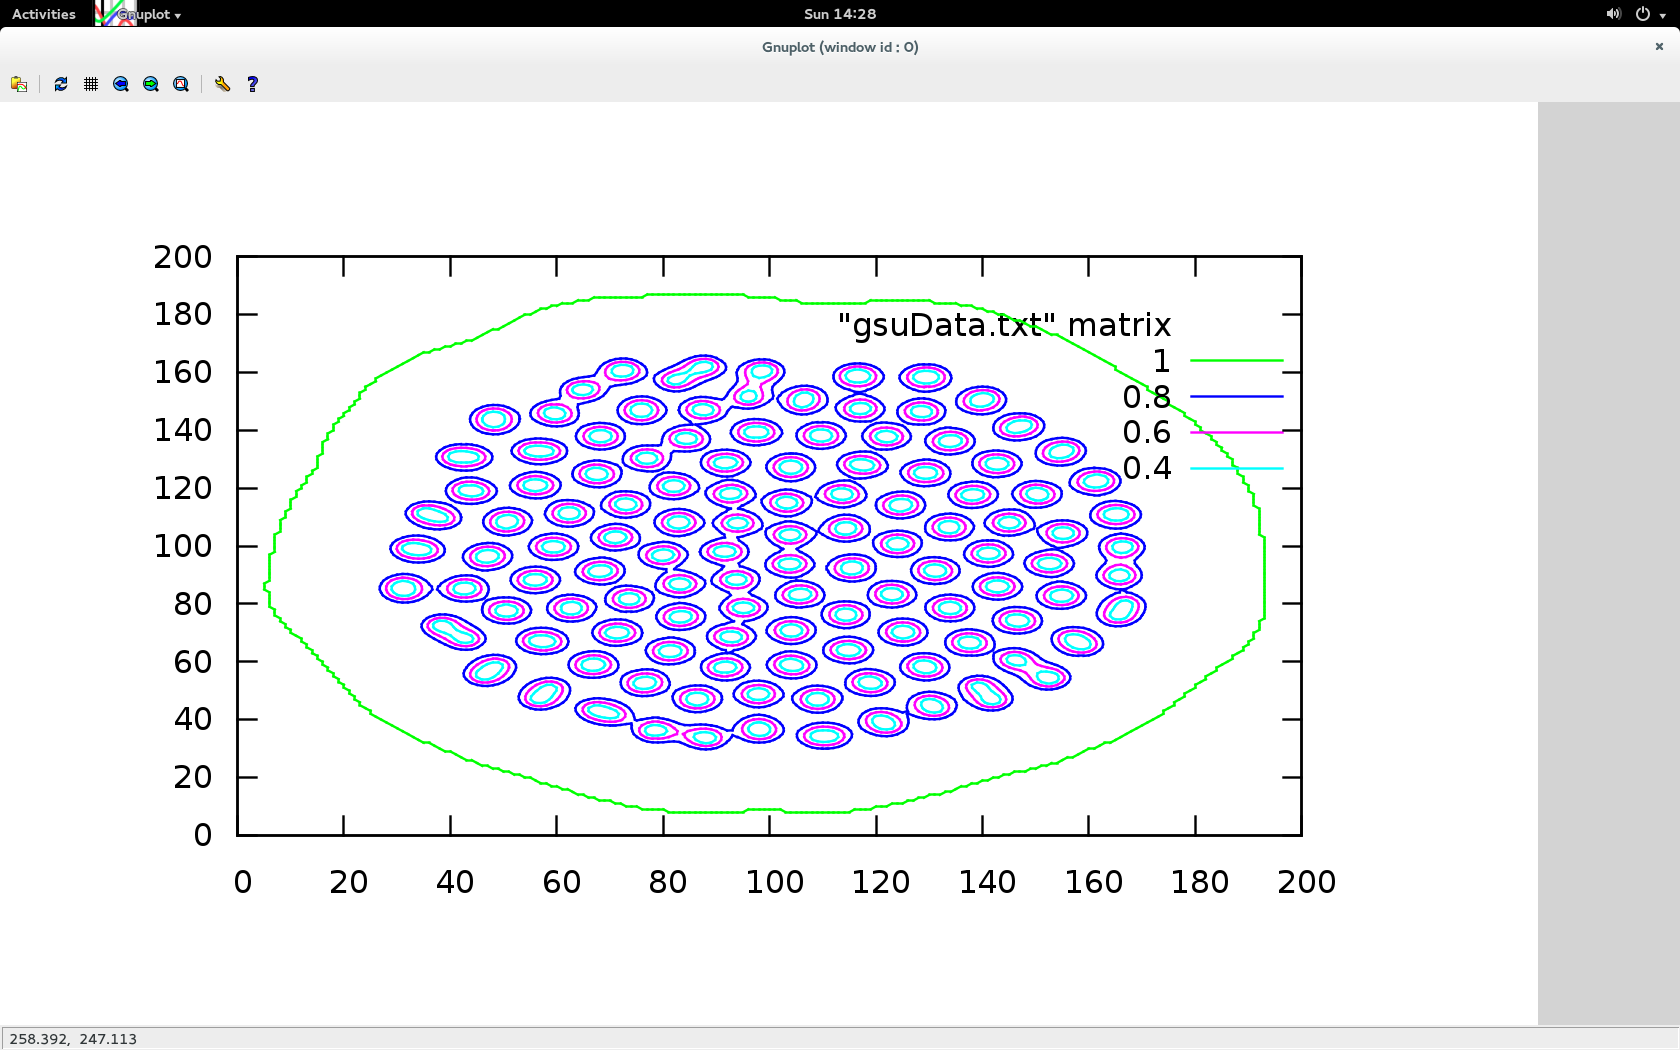
\includegraphics[width=0.75\textwidth]{lambda.png}
\end{center}
\caption{Lambda\label{fig:gprun}}
\end{figure}

\begin{figure}[tbh]
\begin{center}
\includegraphics[width=0.75\textwidth]{Mu.png}
\end{center}
\caption{Mu\label{fig:gprun}}
\end{figure}

\begin{figure}[tbh]
\begin{center}
\includegraphics[width=0.75\textwidth]{Theta.png}
\end{center}
\caption{Theta\label{fig:gprun}}
\end{figure}